%++++++++++++++++++++++++++++++++++++++++
% Don't modify this section unless you know what you're doing!
\documentclass[letterpaper,12pt]{article}
\usepackage{tabularx} % extra features for tabular environment
\usepackage{amsmath}  % improve math presentation
\usepackage{graphicx} % takes care of graphic including machinery
\usepackage[margin=1in,letterpaper]{geometry} % decreases margins
\usepackage[final]{hyperref} % adds hyper links inside the generated pdf file
\hypersetup{
	colorlinks=true,       % false: boxed links; true: colored links
	linkcolor=blue,        % color of internal links
	citecolor=blue,        % color of links to bibliography
	filecolor=magenta,     % color of file links
	urlcolor=blue         
}
%++++++++++++++++++++++++++++++++++++++++

\usepackage{titling}
\pretitle{\begin{flushright}}
\posttitle{\par\end{flushright}}
\preauthor{\begin{flushright}}
\postauthor{\par\end{flushright}}
\predate{\begin{flushright}}
\postdate{\par\end{flushright}}

\usepackage[font=small,skip=0pt]{caption}

% \usepackage[demo]{graphicx}
\usepackage{subcaption}
\usepackage{float}

\usepackage[style=ieee,backend=biber]{biblatex}
\addbibresource{report.bib}

\begin{document}

\title{\vspace{-2cm} Kavi Dey}
\author{\vspace{-0.4cm} E157 RF Design \\ Lab Partner: Zoe Worrall \\ Design Project 1}
\date{\vspace{-0.4cm} \today}
\maketitle

% modified from https://www.overleaf.com/latex/templates/sample-lab-report-for-u-of-r-phys-349/pgsyqngcyjxk
%++++++++++++++++++++++++++++++++++++++++

% abstract
% \begin{abstract}
% abstract here
% \end{abstract}

% sections
\section{Filter Specifications}
% \begin{table}[!ht]
%     \centering
%     \begin{tabularx}{\textwidth}{lX}
%         % \hline
%         % Parameter & Analytical & Simulated w/ ideal components & Simulated w/ real components & Measured \\ \hline
%         % Filter type & Chebyshev I & NA & NA & NA \\ \hline
%         % Filter order & 3 & NA & NA & NA` \\ \hline
%         % Pass Band Edge \newline (defined as exceeding 1dB ripple) & 100 MHz & 100 MHz & ~ & ~ \\ \hline
%         % Stop Band Start \newline (defined @20dB of rejection) & 170 MHz & 173.78 MHz & ~ & ~ \\ \hline
%         % Insertion Loss & 0 dB & 0.0206 dB & ~ & ~ \\ \hline
%         % In-Band Ripple & 0.5 & 0.5210 dB & ~ & ~ \\ \hline
%     \end{tabular}
% \end{table}
\begin{tabularx}{\textwidth}{|l|X|X|X|X|}
    \hline
    Parameter & Analytical & \shortstack{Simulated w/ \\ ideal \\ components} & \shortstack{Simulated w/ \\ real \\ components} & Measured \\
    \hline
    Filter type & Chebyshev I & NA & NA & NA \\
    \hline
    Filter order & 3 & NA & NA & NA \\
    \hline
    \shortstack{Pass Band Edge \\ (defined as exceeding \\ 1dB ripple)} & 99.96 MHz & 100.81 MHz & 98.20 MHz & 96.88 MHz \\
    \hline
    \shortstack{Stop Band Start \\ (defined @ 20dB \\ of rejection)} & 176.06 MHz & 176.88 MHz & 174.17 MHz & 168.84 MHz \\
    \hline
    Insertion Loss & 0.00 dB & 0.02 dB & 0.11 dB & 0.08 dB \\
    \hline
    In-Band Ripple & 0.5 & 0.49 dB & 0.34 dB & 0.36 dB \\
    \hline
\end{tabularx}
\\
\\
\noindent 
\textit{Note:} Due to an issue with the filter table we used which is discussed in the \hyperref[sec:discussion]{Discussions Section}, our pass band edge is at -3 dB, not -1 dB and all measurements are taken at that point.

\newpage
\section{Pictures and Schematics\label{sec:pics_and_schematics}}
% The schematics must be legible, and ltSpice exports often won’t be, so consider redrawing them or adjusting the ltSpice export settings.
% •	A schematic with ideal components
% •	A schematic with real components 
% •	A picture of your assembled circuit
\begin{figure}[H]
    \begin{subfigure}[t]{1\textwidth}
        \centering
        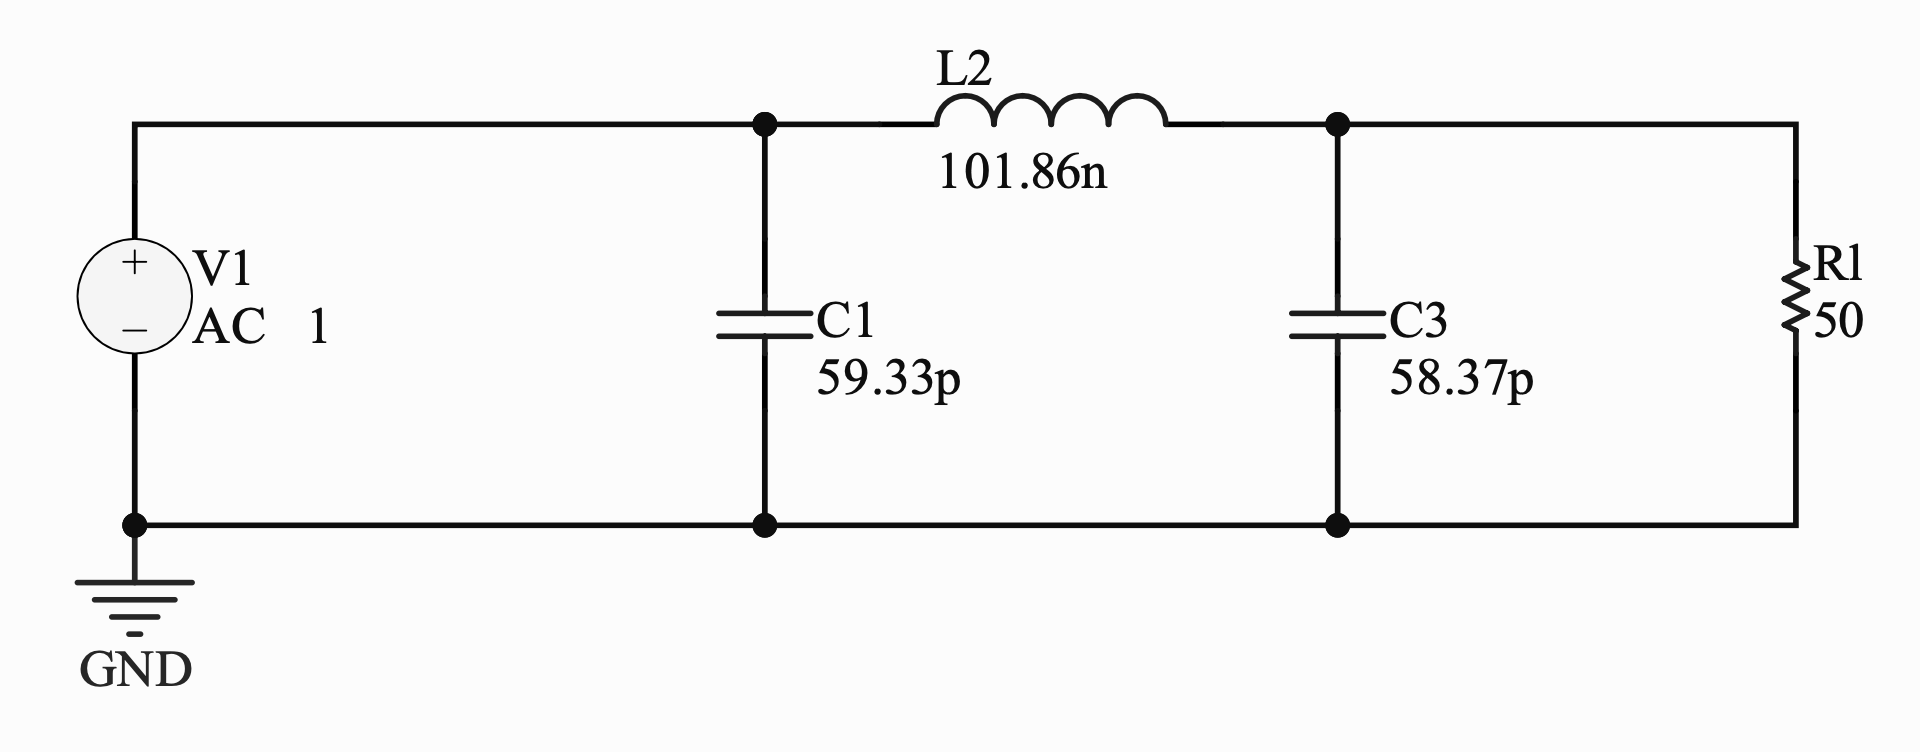
\includegraphics[width=0.8\textwidth]{figures/2.ideal_components}
        \caption{Ideal Components}
    \end{subfigure}

    \medskip

    \begin{subfigure}[t]{1\textwidth}
        \centering
        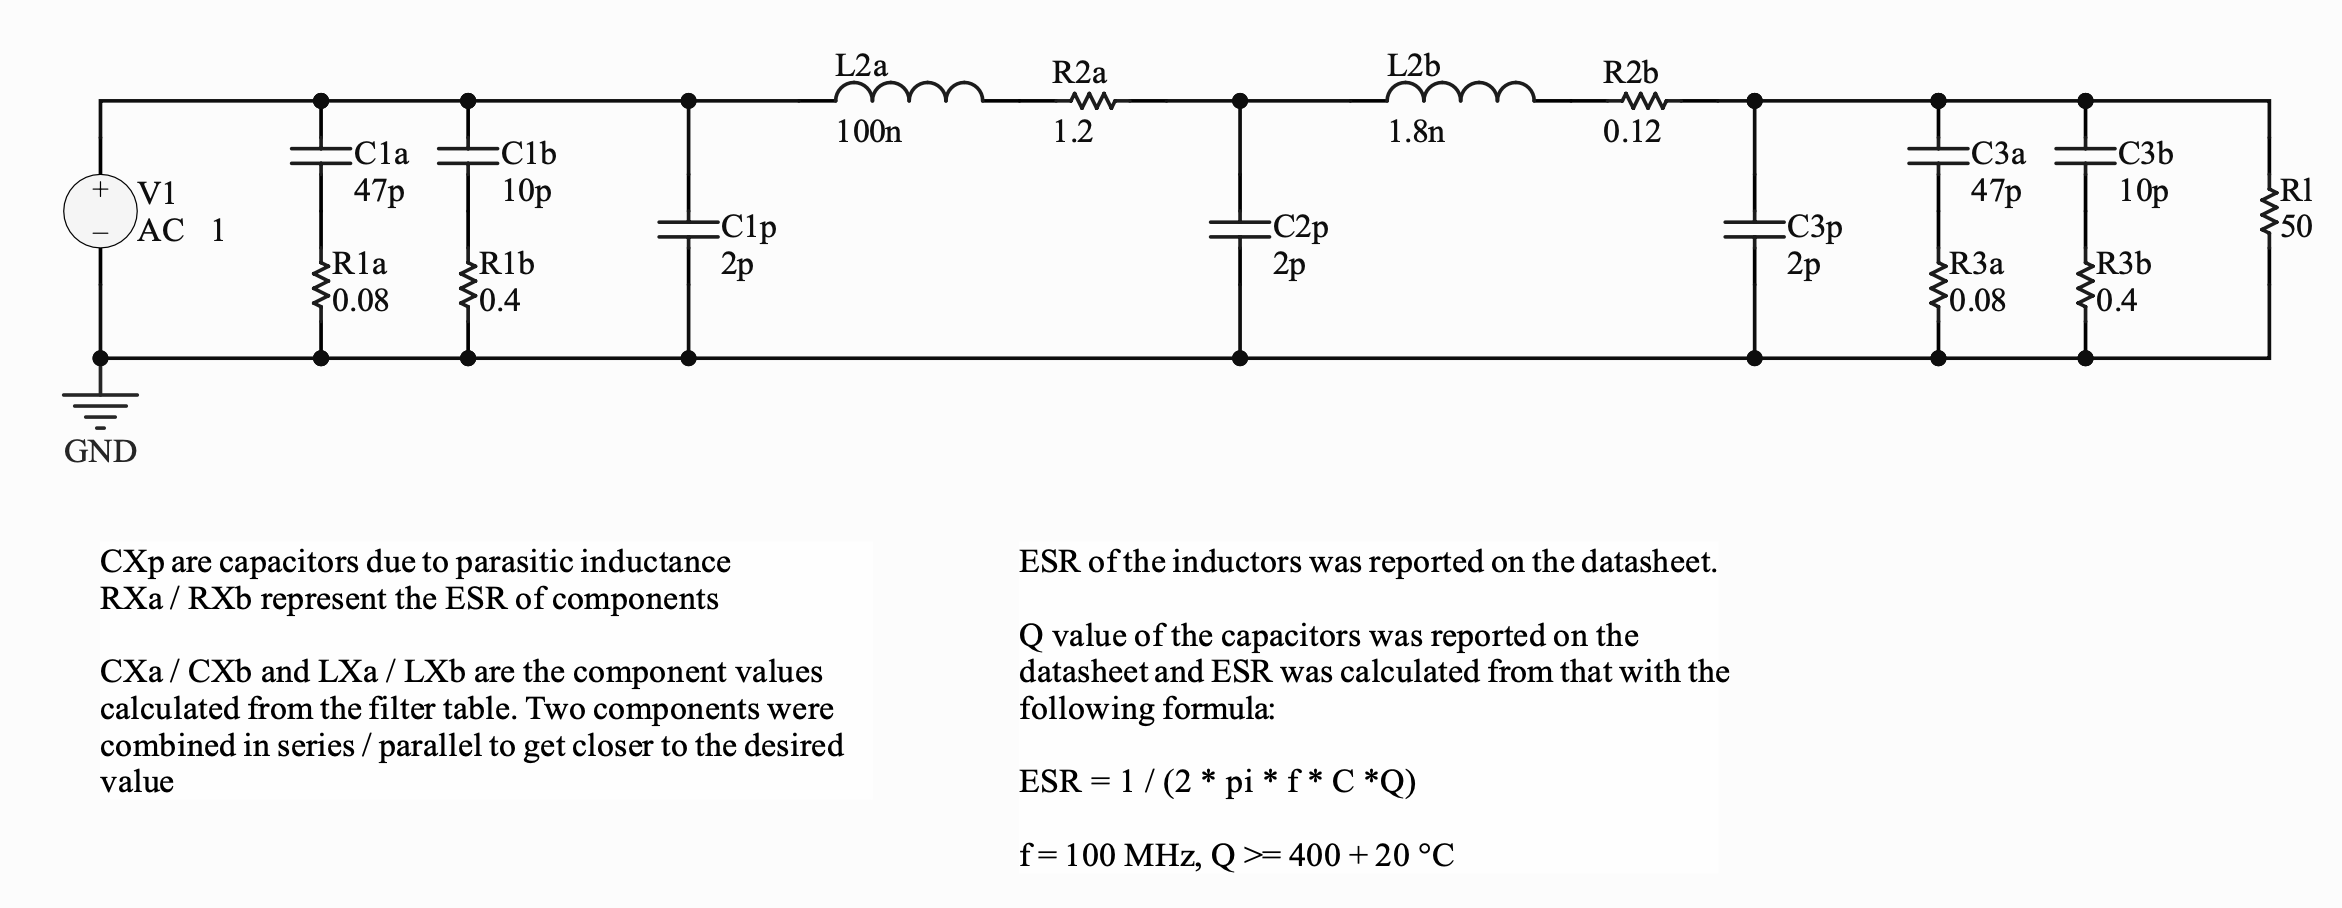
\includegraphics[width=0.8\textwidth]{figures/2.real_components}
        \caption{Real Components}
    \end{subfigure}

    \medskip

    \begin{subfigure}[t]{1\textwidth}
        \centering
        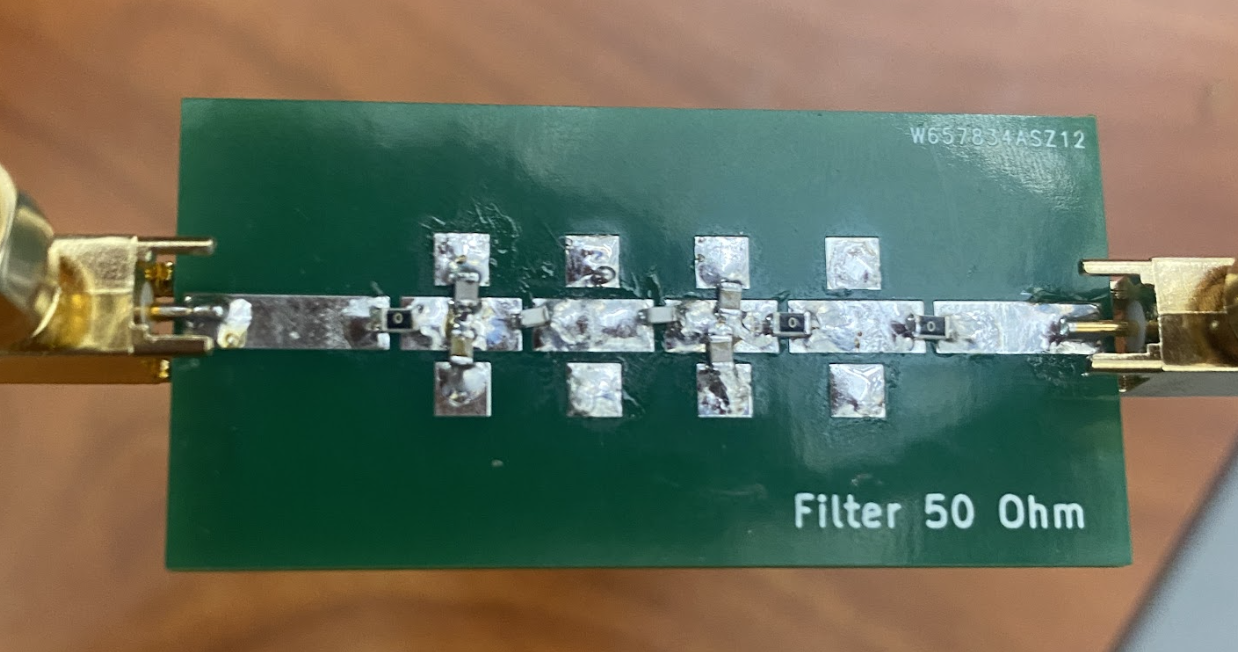
\includegraphics[width=0.8\textwidth]{figures/2.assembled}
        \caption{Assembled Design}
    \end{subfigure}
    \vspace{0.5cm}
    \caption{Simulated and assembled filters}
\end{figure}

\newpage
\section{Hand Calculations\label{sec:hand_calcs}}
% 1-2 pages of hand calculations and tables showing the following.  You may include source code here if it is extremely legible.  You may not just paste a spreadsheet here, but you can include it as a supplementary file for the report.
% •	How you picked your filter type and order including showing
%     o	Your in-band ripple is achievable by your design 
%     o	Your stop-band rejection is achievable by your design
%     o	For Butterworth filters: how you found wp for an in-band ripple of 1dB
% •	The filter table you used (include a citation showing where you found it)
% •	How you synthesized the ideal simulation components using your filter table
% •	Calculation showing power delivered to a 50 Ohm if your filter were driven by a 1Vpp, 0VDC offset, 50 MHz sine wave from a voltage source w/ 50 Ohm output impedance.  You will need your measured insertion loss to complete this calculation, and you may refer to the page in your report where I can check it.
We want to design an LC lowpass filter with an $f_c$ of 100 MHz and minimum attenuation of 20 dB at 200 MHz. The allowable passband ripple is 1 dB and the maximum insertion loss is 3 dB. The source and load resistance are equal at 50 ohms. \\
\\
We can then normalize the attenuation requirements to use attenuation curves:
\begin{align*}
    \frac{f}{f_c} = \frac{200 \text{ MHz}}{100 \text{ MHz}} = 2
\end{align*}
Now we want to select a normalized lowpass filter that offers at least 20 dB of attenuation at a ratio of $f/f_c = 2$.
\begin{figure}[H] 
    \centering 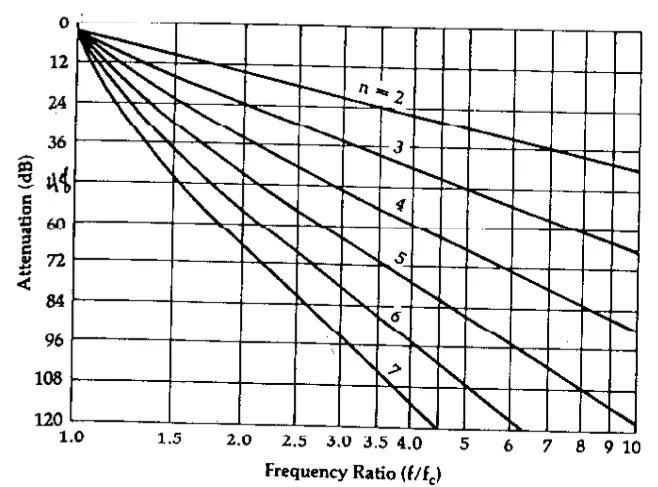
\includegraphics[width=0.5\columnwidth]{figures/3.attenuation_characteristics}
    \caption{
            \label{fig:2.attenuation_characteristics}
            Attenuation characteristics for a Chebyshev filter with 0.5-dB ripple. From RF Circuit Design by Bowick, \cite{Bowick2007-br}
    }
\end{figure}
\noindent
From the attenuation plot, we can see that a 3rd order chebyshev filter has greater than the required attenuation at $f/f_c=2$
% and that the attenuation is equal to 20 dB at $f/f_c \approx 1.7 \implies f_\text{stop band}=170 \text{ MHz}$.
Extracting the point at which there is 20 dB of rejection from the transfer function numerically, we get $f_\text{stop band}=170 \text{ MHz}$. \\
\\
We have chosen to use the 0.5 dB attenuation table, so the expected in band ripple is 0.5 dB.
At the desired stop band, $f = 200 \text{ MHz} \to f/f_c=2$, we can see that there is 24 dB of attenuation.\\
\\
We can predict the attenuation as a function of frequency using
\begin{align*}
    A_\text{dB}=10\log\left[1+\epsilon^2C_n^2\left(\frac{\omega}{\omega_c}\right)'\right]
\end{align*}
Where:
\begin{enumerate}
  \item $\epsilon=\sqrt{10^{R_\text{dB}/10}-1} = 0.3493$ ($R_{dB}$ = 1 dB is the allowable passband ripple)
  \item $\left(\frac{\omega}{\omega_c}\right)' = \left(\frac{\omega}{\omega_c}\right) \cosh B$
  \item $B=\frac{1}{n}\cosh^{-1}\left(\frac{1}{\epsilon}\right)$
  \item $C_3(x)=4x^3-3x$
\end{enumerate}
% Plotting this in python (\href{https://github.com/kavidey/e157/blob/main/dp_01/predict_chebyshev.py}{code link}) we get:
% \begin{figure}[ht] 
%     \centering 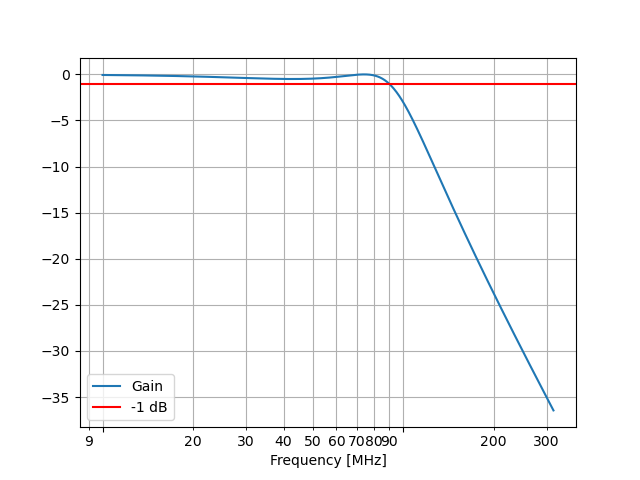
\includegraphics[width=0.5\columnwidth]{figures/3.mag}
%     \caption{
%             \label{fig:2.mag}
%             Attenuation characteristics for a Chebyshev filter with 0.5-dB ripple.
%     }
% \end{figure}
% Extracting the pass band ripple from the graph we get 0.5 dB, as predicted from the filter table in figure \ref{fig:2.filter_table}
The following table can be used to calculate component values for $n=3$ and $R_S/R_L = 1$ as follows:
\begin{figure}[H] 
    \centering 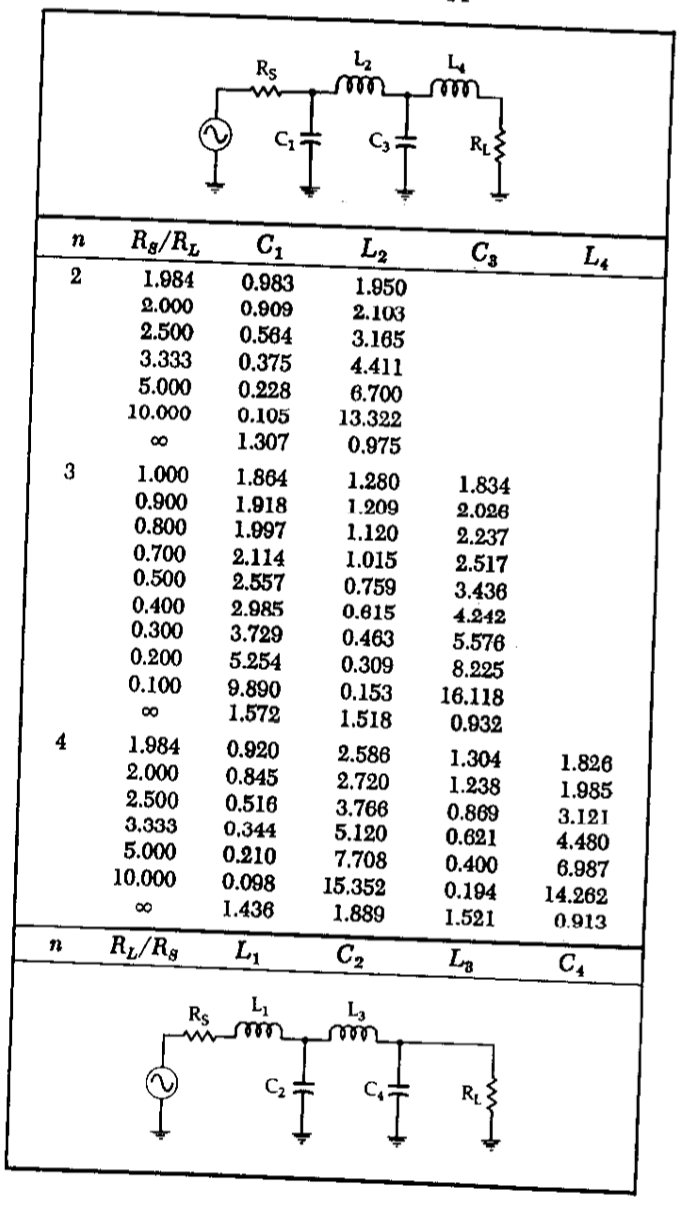
\includegraphics[width=0.3\columnwidth]{figures/3.filter_table}
    \caption{
            \label{fig:2.filter_table}
            Chebyshev Low-Pass Prototype Element Values for 0.5-dB Ripple.  From RF Circuit Design by Bowick, \cite{Bowick2007-br}
    }
\end{figure}
\noindent
Plugging in we get:
\begin{align*}
    C_1 = \frac{1.864}{2\pi(100\times10^6)50} = 59.33 \text{ pF} \\
    L_2 = \frac{(1.280)(50)}{2\pi(100\times10^6)} = 101.86 \text{ nH} \\
    C_3 = \frac{1.834}{2\pi(100\times10^6)50} = 58.37 \text{ pF}
\end{align*}
Because we are making a lowpass filter, we can use the provided schematic as is. We have chosen to use the \textbf{top} schematic in Figure \ref{fig:2.filter_table}. \\
\\
Calculation showing power delivered to a 50 Ohm if your filter were driven by a 1 Vpp, 0 VDC offset, 50 MHz sine wave from a voltage source w/ 50 Ohm output impedance.\\
\\
The input wave has a power of
$$P=\left(\frac{1 \ V}{2\sqrt{2}}\right)^2 \frac{1}{50 \Omega} = 2.5 \text{ mW} \approx 4 \text{ dBm}$$
The report instructions say to assume that the only loss is due to insertion loss, however for the filter we built the attenuation at 50 MHz is significantly more than just insertion loss. Therefore we are providing two calculations for delivered power, one assuming just insertion loss and one with the true loss at 50 Mhz. See page \pageref{sec:s21_dcstop} for insertion loss measurement and \pageref{sec:s21_pass} for the 50 MHz loss. \\
\\
In general the total power delivered into the load is:
$$\text{Dissipated Power} = 4 \text{ dBm} - \text{Insertion Loss}$$
Using only insertion loss:
$$4 \text{ dBm} - 0.08 \text{ dB} = 3.92 \text{ dBm} \approx 3.47 \text{ mW} $$
Using 50 MHz loss:
$$4 \text{ dBm} - 0.93 \text{ dB} = 3.07 \text{ dBm} \approx 2.02 \text{ mW} $$

\newpage
\section{Magnitude of S21 in Pass band\label{sec:s21_pass}}
% Magnitude of S21 in your pass band for all four designs
% •	Use the frequency range 40MHz-130MHz.  Display in on a linear scale.
% •	Use dB as your y-axis units
% •	Do not overlay these graphs.  Please include four of them in a 2x2 grid.
% •	Each representation needs to include annotated markers that show the magnitude and frequency of 
%     o	The maximum value in the pass band
%     o	The minimum ripple value in the pass band
%     o	The pass band edge. (In a Butterworth or Chebyshev II filter, this might be the same marker as the minimum ripple value.)
\begin{figure}[H]
    \begin{subfigure}[t]{.49\textwidth}
      \centering
      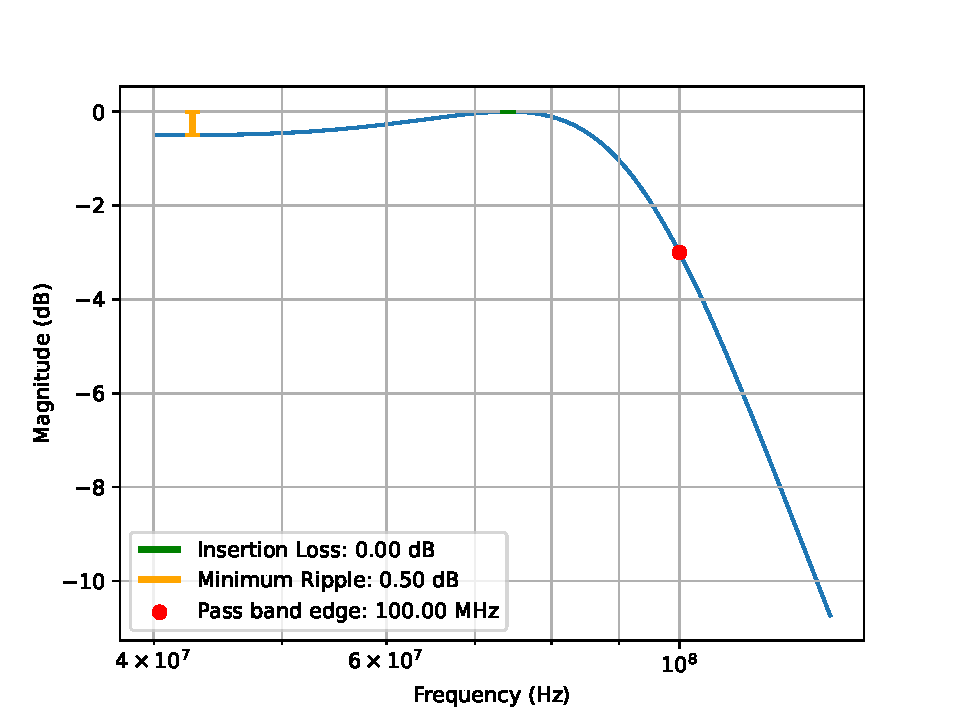
\includegraphics[width=\linewidth]{figures/4.analytical}
      \caption{Analytical Design}
    \end{subfigure}
    \hfill
    \begin{subfigure}[t]{.49\textwidth}
      \centering
      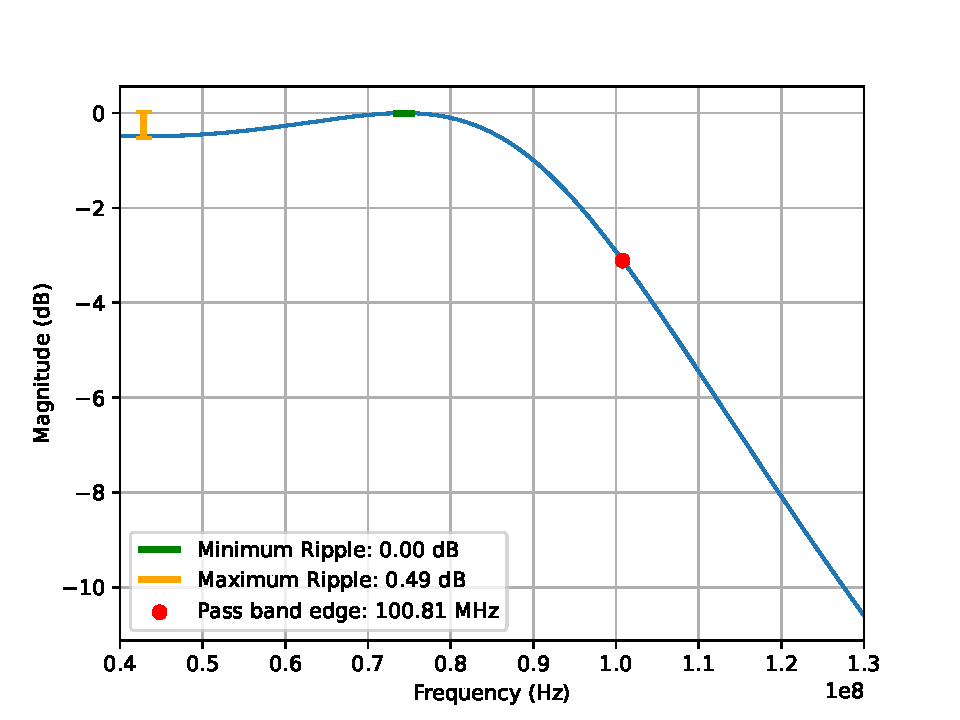
\includegraphics[width=\linewidth]{figures/4.ideal}
      \caption{Simulated design with ideal components}
    \end{subfigure}
  
    \medskip
  
    \begin{subfigure}[t]{.49\textwidth}
      \centering
      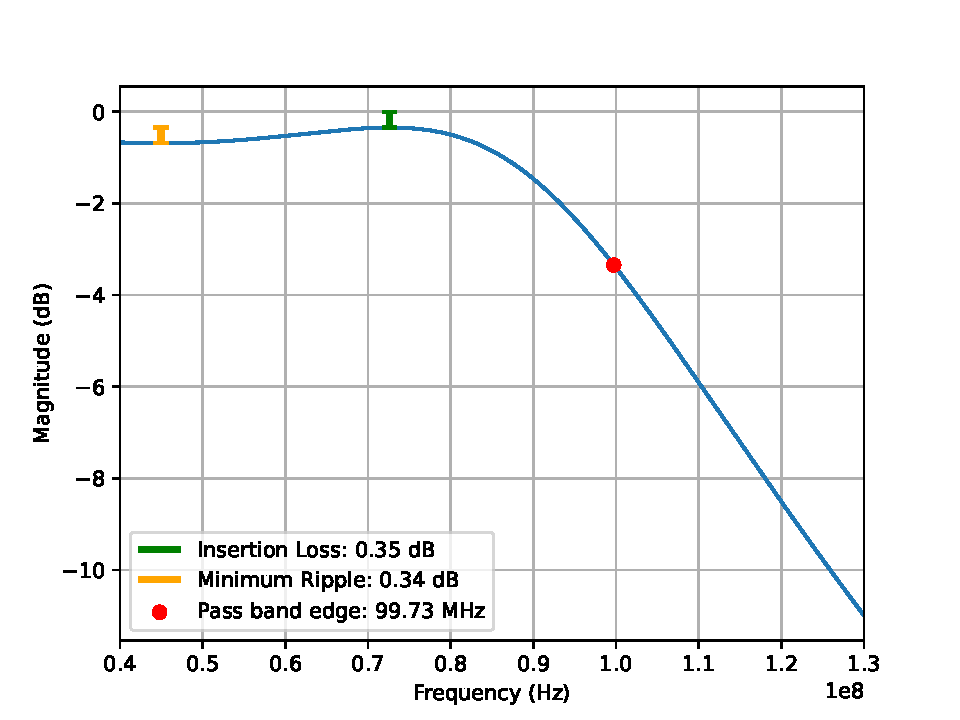
\includegraphics[width=\linewidth]{figures/4.real}
      \caption{Simulated Design with real components}
    \end{subfigure}
    \hfill
    \begin{subfigure}[t]{.49\textwidth}
      \centering
      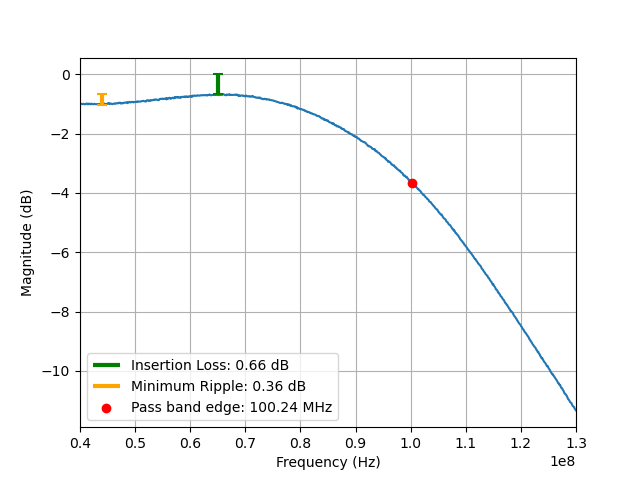
\includegraphics[width=\linewidth]{figures/4.assembled}
      \caption{Assembled Design}
    \end{subfigure}

    \vspace{0.5cm}
    \caption{S21 Pass band for all filters with annotations}
  \end{figure}

\newpage
\section{Phase of S21 in Pass band\label{sec:phase}}
% Phase of S21 in your pass band for three designs: the ideal simulation, the real simulation and the measured design.
% •	Use the frequency range 40MHz-130MHz.  Display in on a linear scale.
% •	Use degrees between -180/+180 as your y-axis units (i.e.: provide a wrapped phase plot)
% •	Overlay these graphs on one frequency axis.
% •	Each representation needs to include one annotated marker at the band edge (which you found from your magnitude plot) that shows the phase and frequency.
\begin{figure}[H]
    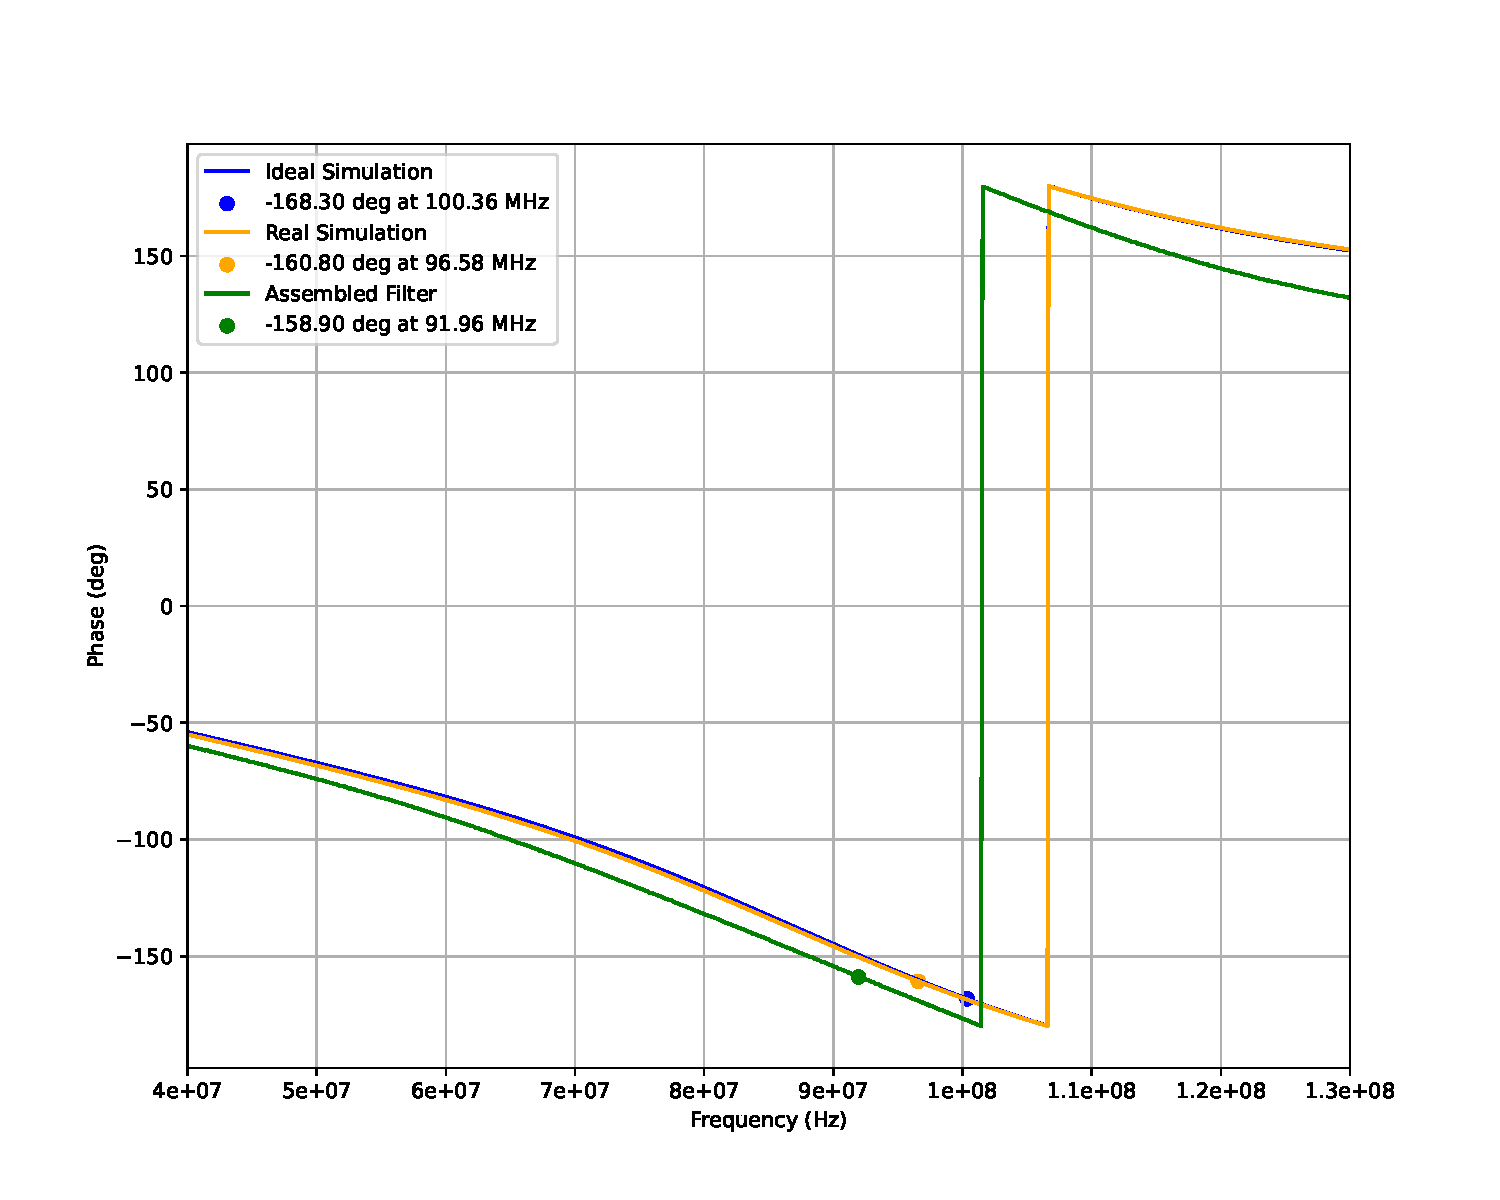
\includegraphics[width=\linewidth]{figures/5.phase}
    \caption{Phase of S21 in Pass band for ideal simulation, real simulation, and assembled design}
\end{figure}

\newpage
\section{Magnitude of S21 from DC to Stop band\label{sec:s21_dcstop}}
% Magnitude of S21 from DC to your stop band for all four designs
% •	Use the frequency range 0Hz to 300MHz (or as low as the instrument will go for measurements).  Display your frequency range on a log scale.
% •	Use dB as your y-axis units.
% •	Do not overlay these graphs.  Please include four of them in a 2x2 grid.
% •	Each representation needs to include annotated markers that show the magnitude and frequency of 
%     o	The value of insertion loss in the pass band (i.e.: the “DC” value of S21)
%     o	The pass band edge
%     o	The stop band edge.
\begin{figure}[H]
    \begin{subfigure}[t]{.49\textwidth}
      \centering
      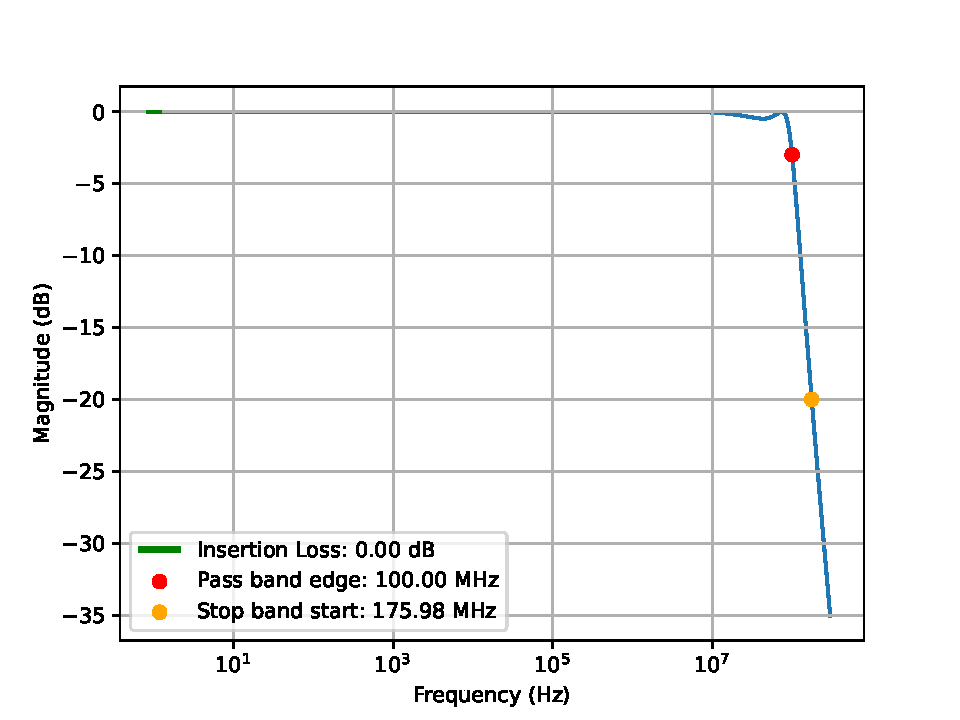
\includegraphics[width=\linewidth]{figures/6.analytical.pdf}
      \caption{Analytical Design}
    \end{subfigure}
    \hfill
    \begin{subfigure}[t]{.49\textwidth}
      \centering
      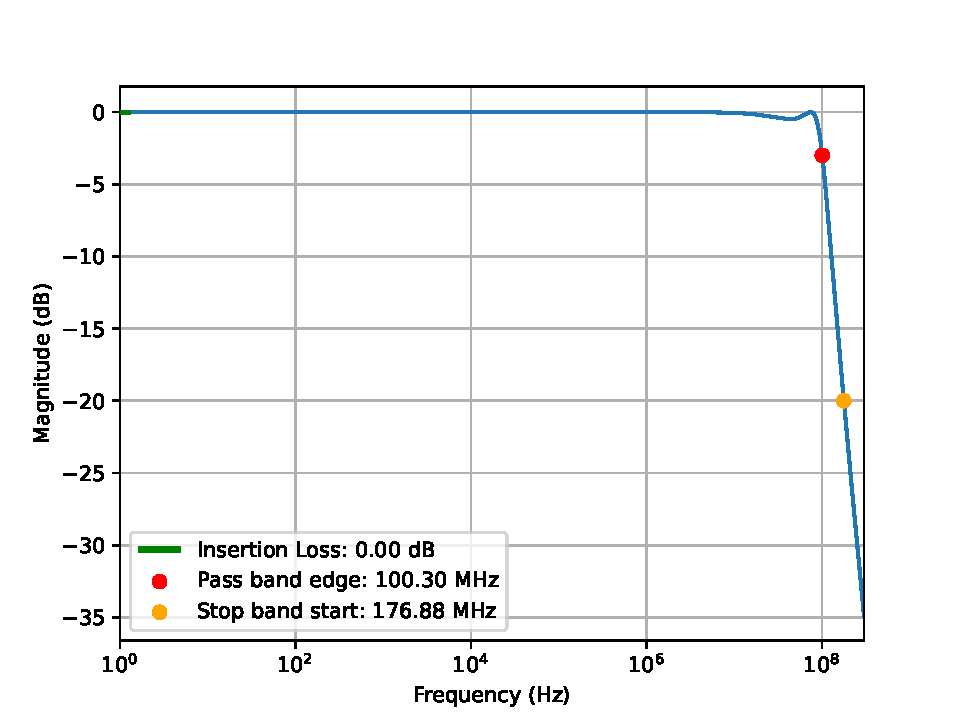
\includegraphics[width=\linewidth]{figures/6.ideal}
      \caption{Simulated design with ideal components}
    \end{subfigure}
  
    \medskip
  
    \begin{subfigure}[t]{.49\textwidth}
      \centering
      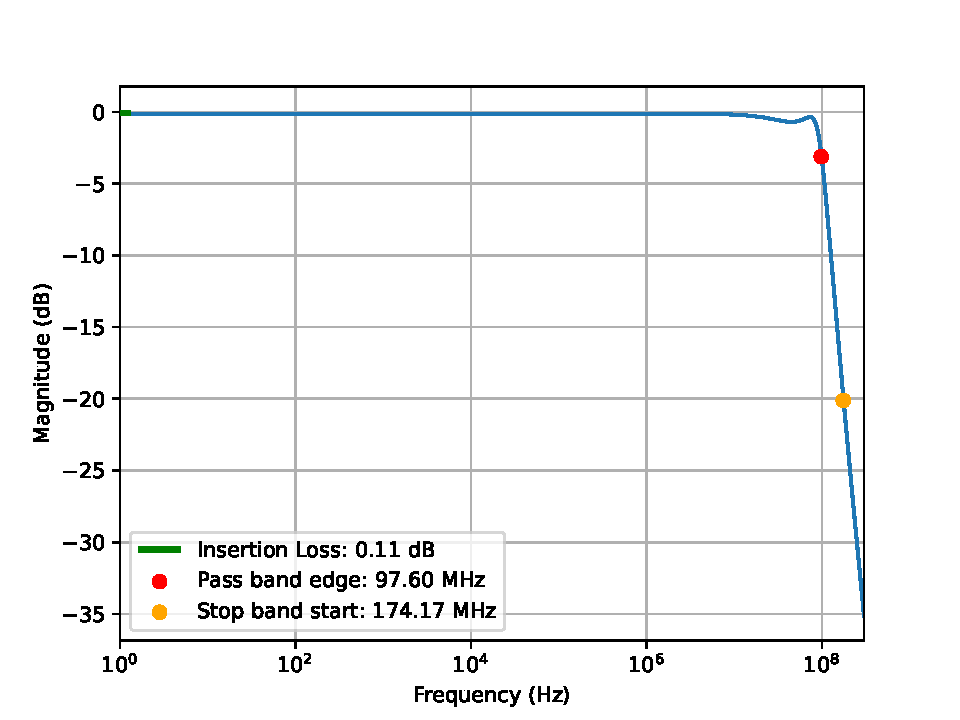
\includegraphics[width=\linewidth]{figures/6.real}
      \caption{Simulated Design with real components}
    \end{subfigure}
    \hfill
    \begin{subfigure}[t]{.49\textwidth}
      \centering
      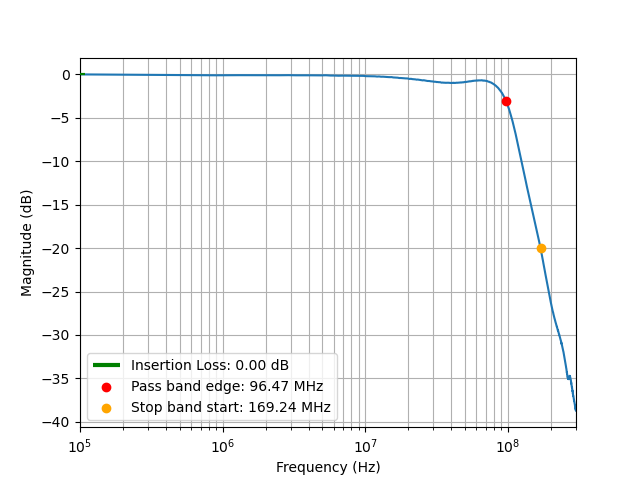
\includegraphics[width=\linewidth]{figures/6.assembled}
      \caption{Assembled Design}
    \end{subfigure}
    \vspace{0.5cm}
    \caption{S21 DC to Stop band for all filters with annotations}
  \end{figure}

\newpage
\section{Magnitude of S11 from DC to Stop band\label{sec:s11}}
% Magnitude of S11 from DC to your stop band for all four designs.  Note that for the analytical design you will need to derive this from your S21 magnitude and power conservation.
% •	Use the frequency range 0Hz to 300MHz (or as low as the instrument will go for measurements).  Display your frequency range on a log scale.
% •	Use dB as your y-axis units.
% •	Do not overlay these graphs.  Please include four of them in a 2x2 grid.
% •	Each representation needs to include annotated markers that show the magnitude and frequency of 
%     o	The pass band edge
%     o	The stop band edge.
\begin{figure}[H]
    \begin{subfigure}[t]{.49\textwidth}
      \centering
      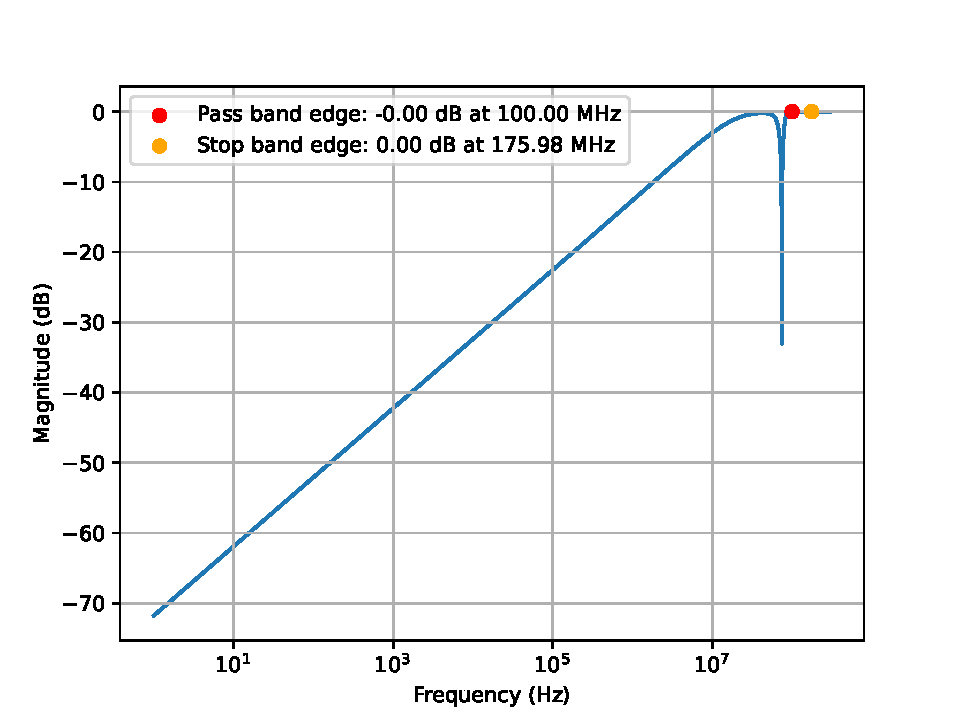
\includegraphics[width=\linewidth]{figures/7.analytical}
      \caption{Analytical Design}
    \end{subfigure}
    \hfill
    \begin{subfigure}[t]{.49\textwidth}
      \centering
      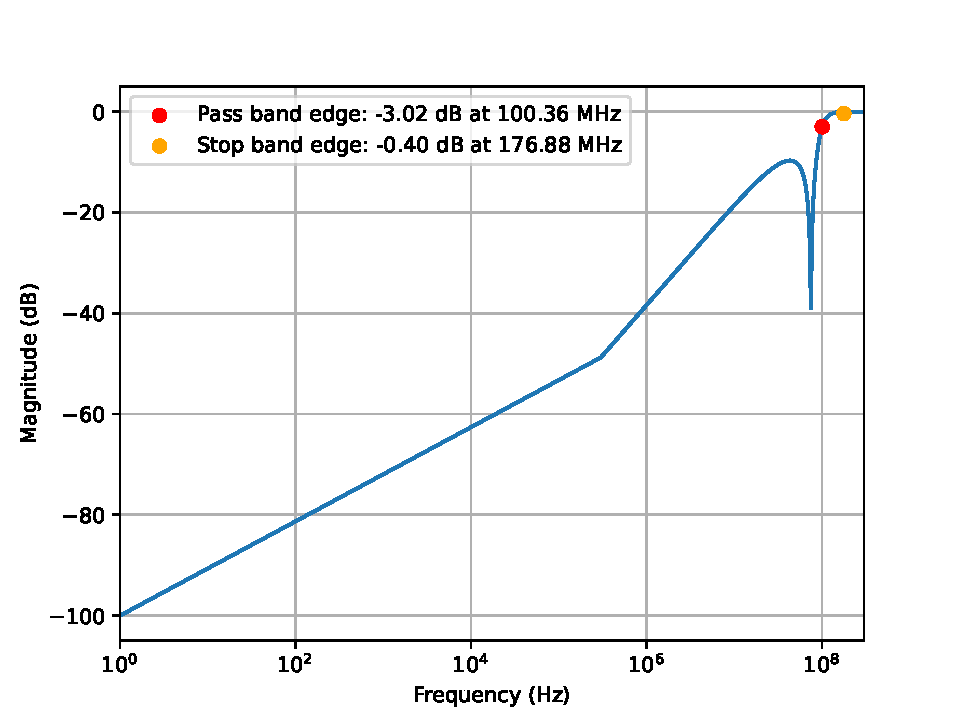
\includegraphics[width=\linewidth]{figures/7.ideal}
      \caption{Simulated design with ideal components}
    \end{subfigure}
  
    \medskip
  
    \begin{subfigure}[t]{.49\textwidth}
      \centering
      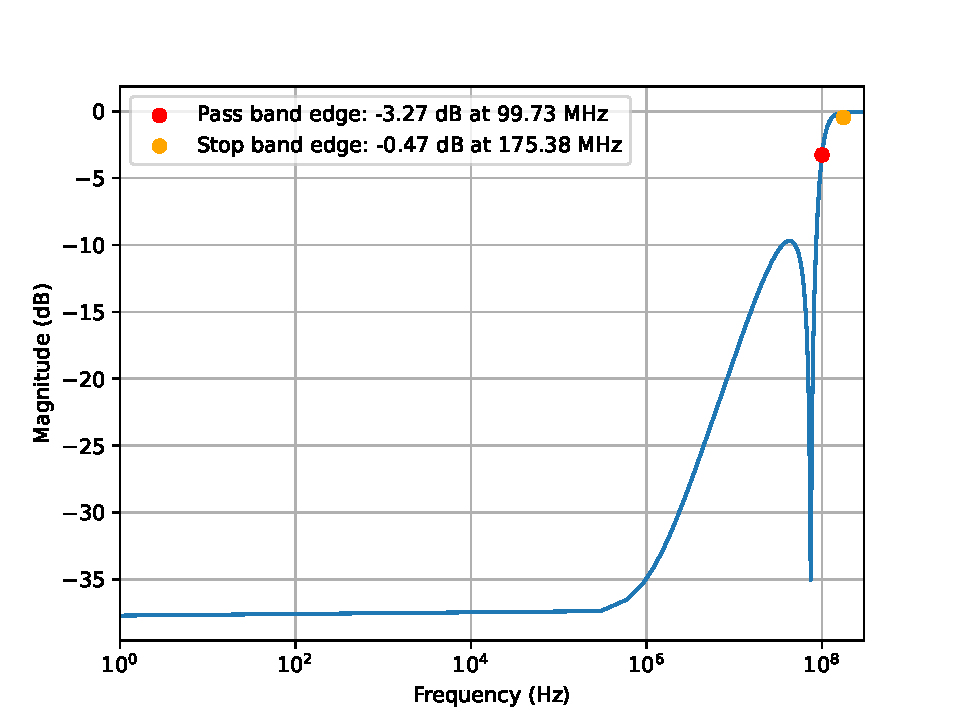
\includegraphics[width=\linewidth]{figures/7.real}
      \caption{Simulated Design with real components}
    \end{subfigure}
    \hfill
    \begin{subfigure}[t]{.49\textwidth}
      \centering
      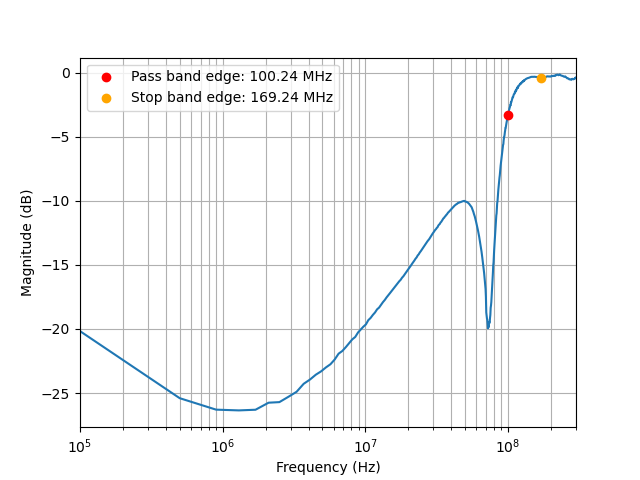
\includegraphics[width=\linewidth]{figures/7.assembled}
      \caption{Assembled Design}
    \end{subfigure}
    \vspace{0.5cm}
    \caption{S11 from DC to Stop band for all filters with annotations}
  \end{figure}

\newpage
\section{Smith Charts for S11 and S21 from DC to Stop band\label{sec:smith}}
% Smith Charts for S11 and S21 from DC to your stop band for three designs: the ideal simulation, the real simulation and the measured results.  Use the frequency range 0Hz to 300MHz and do not overlay the graphs, instead arranging them in a 3x2 grid with S11 on the left.
\begin{figure}[H]
    \begin{subfigure}[t]{.49\textwidth}
        \centering
        S11
    \end{subfigure}
    \hfill
    \begin{subfigure}[t]{.49\textwidth}
        \centering
        S21
    \end{subfigure}
    
    \begin{subfigure}[t]{.49\textwidth}
      \centering
      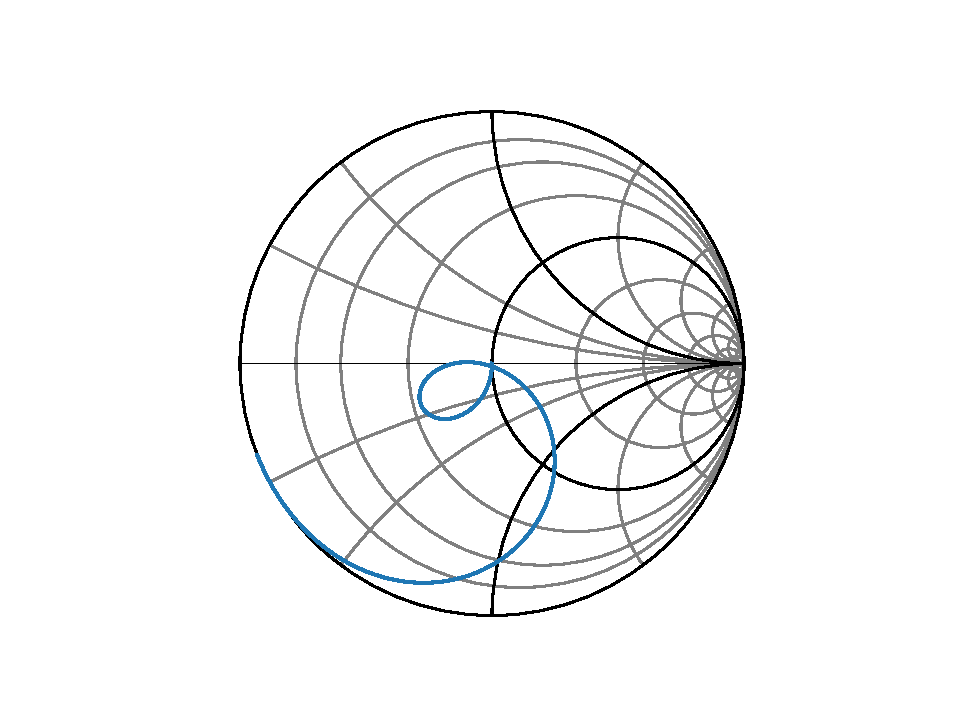
\includegraphics[width=\linewidth]{figures/8.s11.ideal}
      \caption{Ideal Simulation S11}
    \end{subfigure}
    \hfill
    \begin{subfigure}[t]{.49\textwidth}
      \centering
      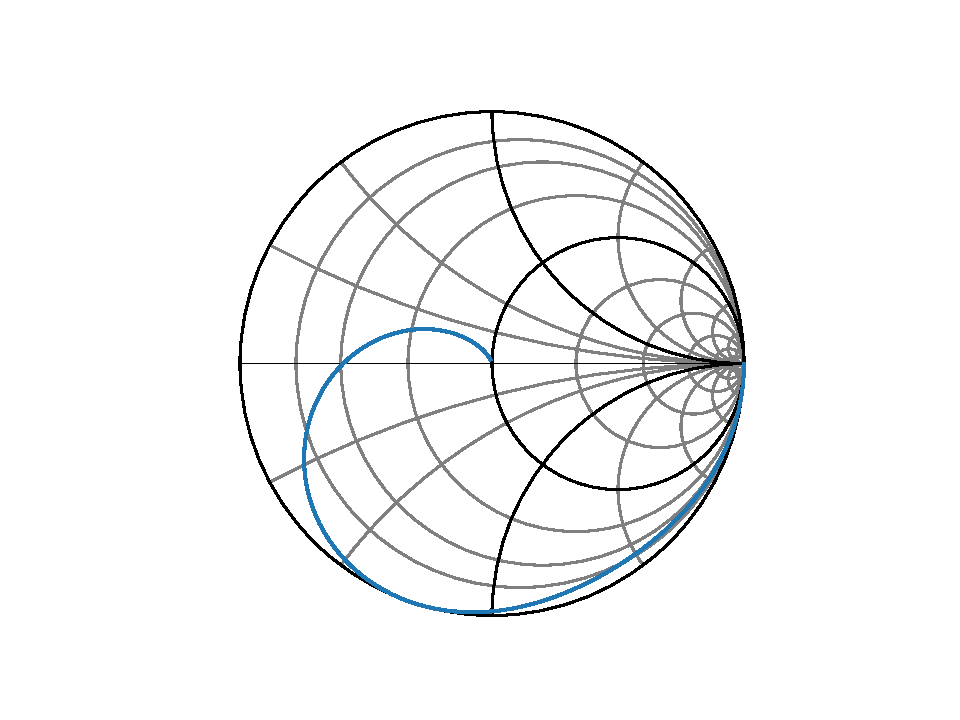
\includegraphics[width=\linewidth]{figures/8.s21.ideal}
      \caption{Ideal Simulation S21}
    \end{subfigure}
    
    \begin{subfigure}[t]{.49\textwidth}
      \centering
      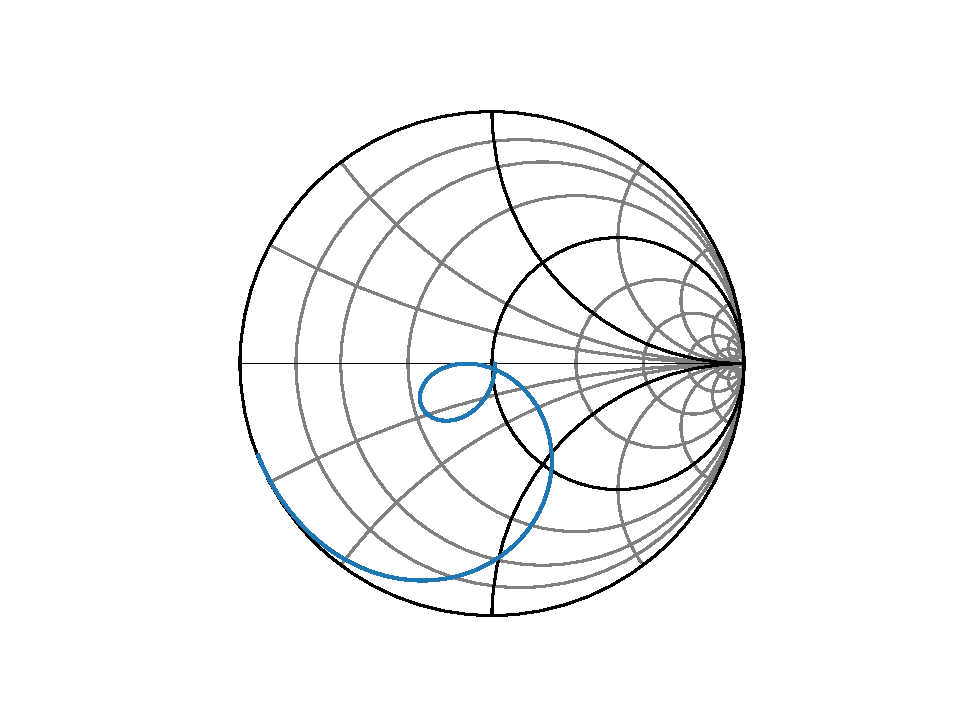
\includegraphics[width=\linewidth]{figures/8.s11.real}
      \caption{Real Simulation S11}
    \end{subfigure}
    \hfill
    \begin{subfigure}[t]{.49\textwidth}
      \centering
      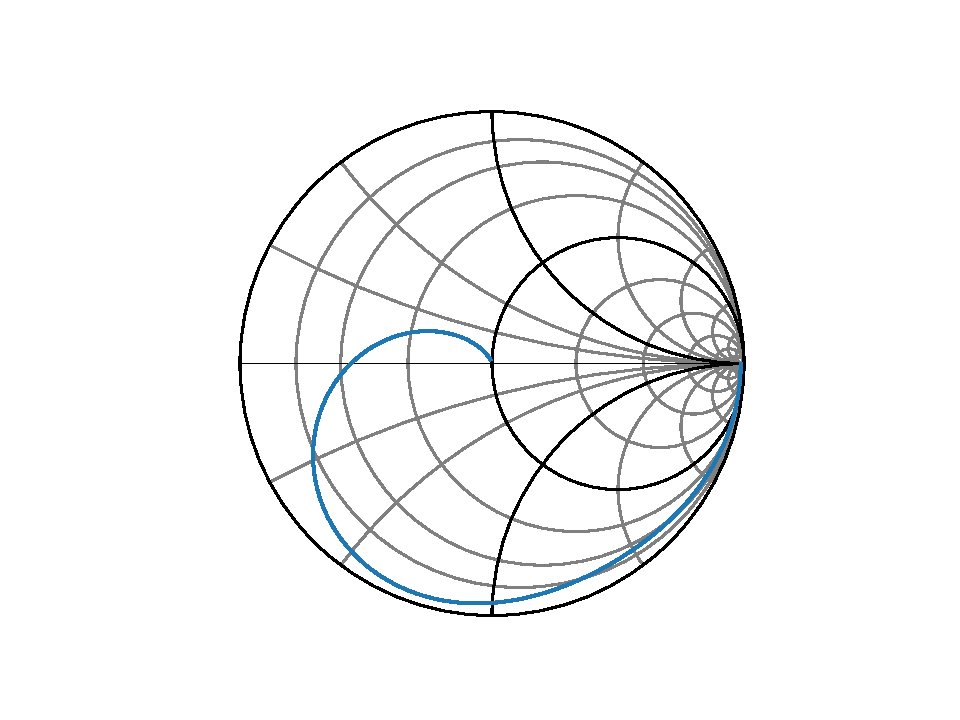
\includegraphics[width=\linewidth]{figures/8.s21.real}
      \caption{Real Simulation S21}
    \end{subfigure}
  
    \begin{subfigure}[t]{.49\textwidth}
      \centering
      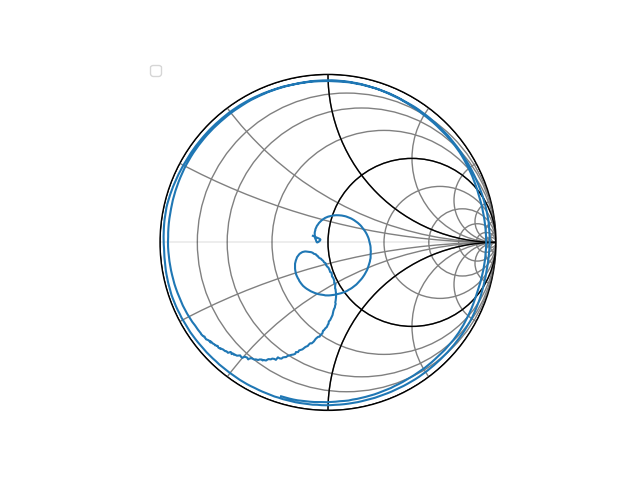
\includegraphics[width=\linewidth]{figures/8.s11.assembled}
      \caption{Assembled Design S11}
    \end{subfigure}
    \hfill
    \begin{subfigure}[t]{.49\textwidth}
      \centering
      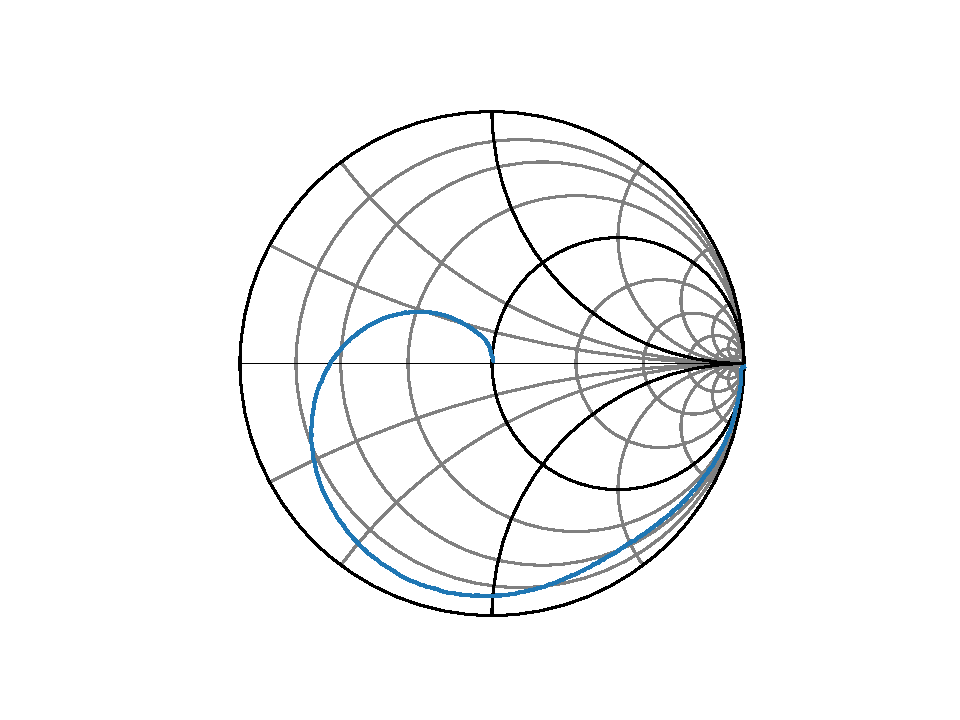
\includegraphics[width=\linewidth]{figures/8.s21.assembled}
      \caption{Assembled Design S21}
    \end{subfigure}
    \vspace{0.5cm}
    \caption{S11 and S22 Smith charts for simulated ideal, real, and assembled filters}
\end{figure}

\newpage
\section{Discussions \label{sec:discussion}}
% Discussion of discrepancies between analytical, simulated and measured results.  Quantitatively justify differences between them, including any modifications you made to your models to make your simulations match your measurements better (e.g.: board parasitics).  Refer to prior figures in your report for supporting evidence in this discussion.
\subsection{Filter Table Passband Edge Issue}
The Chebyshev I filter design table we used when designing our filter was created to have 3 dB of attenuation at the passband edge, not 1 dB as desired. Unfortunately, we didn't realize this until after we had already built and measured our filter. We were told that we didn't need to make a new filter, but that we should discuss how we would change our math in section \ref{sec:hand_calcs} to account for this discrepancy.
\\
\\
Unlike with a Butterworth filter, it is not possible to analytically calculate the adjusted corner frequency to get 1 dB attenuation. Instead we searched the parameter space programatically to determine that we need to use an adjusted $f_c = 111.44 \text{ MHz}$ to get 1 dB attenuation at 100 MHz. 
By increasing the corner frequency, we are effectively shifting the whole transfer function ``right'' on the frequency axis, so we need to confirm that a 3rd order Chebyshev I filter still has enough attenuation at 200 MHz to fulfill the filter requirements. Analytically calculating the stop band start we get 196.0 MHz which is lower than the specification of 200 MHz confirming that a 3rd order Chebyshev I filter has a fast enough falloff even with the adjusted corner frequency. Re-doing the component calculations with these new values we get: $C_1 = 53.24 \text{ pF}, L_2 = 91.40 \text{ nH}, C_3 = 52.38 \text{ pF}$ which are reasonably close to the values we used in or 3 dB attenuation filter. \\
\\
To keep values consistent with the expected 100 MHz value, all pass band edge frequencies are calculated with \textbf{3 dB} of attenuation instead of 1 dB.
% (1.280*50)/(2*pi*111.439e6)
% Issue: the table assumed that we wanted the corner frequency to be at -3db, not -1db as the filter specs say.
% Inspecting the analytical Chebyshev 1 attenuation plot, we find that we would need to adjust f_c from 100 MHz to 111.5 MHz for the attenuation to be 1db at 100 MHz. This would result in a stop band edge of 196.1 MHz, which is still within the desired filter parameters.
\subsection{Matching between Analytical and Ideal Simulation}
The analytical filter predicted by the Chebyshev I polynomial matches the simulation with ideal components (Figure \hyperref[sec:pics_and_schematics]{1a}) very closely. The passband edge and stop band frequencies are very similar (to within margin of measurement error) and the insertion loss and in-band ripple match almost exactly. This makes sense and is expected as the simulation with ideal components should have a perfect match to the predicuted Chebyshev I polynomial. In addition to specific S21 measurements, the general shape also matches fairly closely (see Figures \ref{sec:s21_pass} and \ref{sec:s21_dcstop}). Analytical S11 was calculated using power conservation ($|S_{11}|^2 + |S_{21}|^2 = 1$) and the shape and location of resonant dip in the analytical and ideal simulation are fairly close (Figure \ref{sec:s11}).
\subsection{Accounting for Board and Component Parasitics in Real Design and Simulation}
There are two sources of parasitic impedance that we accounted for when constructing the filter. The first is parasitic capacitance and inductance from the pads and vias on the filter board as shown in Figure \ref{fig:9.board_parasitics}.

\begin{figure}[H]
  \centering 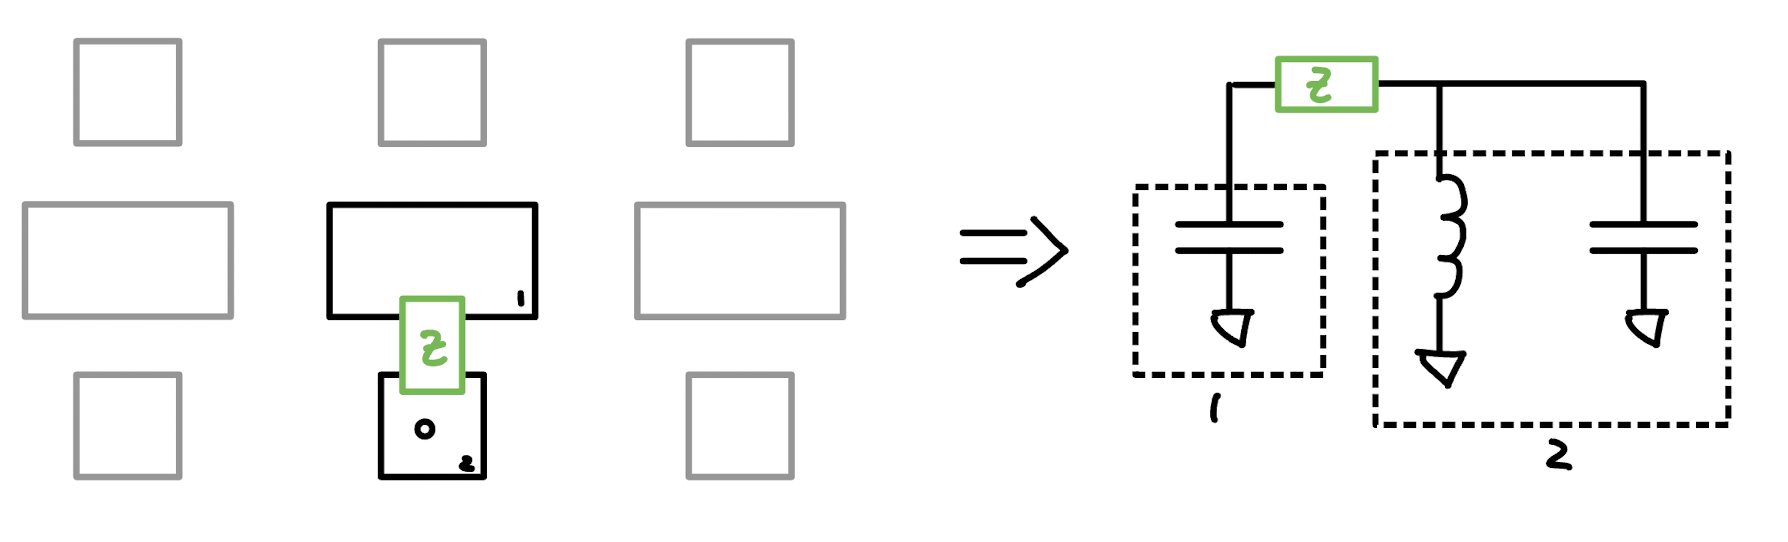
\includegraphics[width=0.7\textwidth]{figures/9.parasitics}
  \caption{Diagram of filter board parasitics \label{fig:9.board_parasitics}}
\end{figure}
\noindent
Parasitic capacitance is due to the parallel plate capacitor formed by the metal pads on either side of the PCB, and parasitic inductance is caused by loops formed by vias connecting pads from the top layer to ground on the bottom layer. The second is the ESR of the capacitors and inductors that were used to build the filter. In Lab 3, we performed parasitic extraction on the filter boards and determined that the parasitic inductance is around 10 nH and the parasitic capacitance is around 2 pF. For components that did not list an ESR value, we calculated it from the Q value using the process defined in Section \ref{sec:pics_and_schematics}, Figure \hyperref[sec:pics_and_schematics]{1b}.
\\
\\
We don't have access to higher Q components, so we have no easy way to combat ESR. To account for the parasitic pad capacitance, we reduced the values of the capacitors on the filter board by 2 pF so that total capacitance adds up to the desired value. Figure 1b shows the modifications made to the ideal schematic to account for parasitics.
\subsection{Analysis of Differences Between Four Filters}
I have talked above about the close similarities between analytical prediction and ideal simulation, so I am focusing on the similarities and differences between ideal simulation, real simulation, and assembled filter for this portion.
\\
\\
Overall, the three filters match very closely. The magnitude of S21 from DC to stop band in Figure \ref{sec:s21_dcstop} look almost identical. All four designs have stop bands in similar locations (176 to 177 MHz for analytical and ideal sim, 174 MHz for real sim, and 168 MHz for analytical filter). It is important to note that the frequency resolution of the VNA is not very high. It only captures 751 points between 100 kHz and 300 MHz and the frequency jumps between points is on the order of 1 MHz.
\\
\\
The magnitude of S21 in the passband (Figure \ref{sec:s21_pass}) has a similar shape, with the exception that real simulation and assembled filter have a less-tall peak due to losses from parasitic component ESR. Interestingly, the ripple in the real simulation and assembled filter is also less than that predicted by the ideal simulation (0.34 dB, 0.36 dB, and 0.5 dB respectively), likely due to component variations. Another area of importance is the passband edge, all of which are within 4 MHz of the 100 MHz target (Figure \ref{sec:s21_pass}). The real and ideal simulations are closest at 98.20 and 100.81 MHz. The assembled filter as a slightly lower pass band edge of 96.88 MHz. This lower pass band edge is due to a combination of factors including component variation and VNA frequency measurement error.
\\
\\
The S21 phase of all three signals also have a very similar shape as seen in Figure \ref{sec:phase}. The ideal and real simulations match almost perfectly, while the assembled filter has a very similar shape, shifted left on the frequency axis. This shift is due to additional phase picked up throughout the length of the filter PCB. The PCB is 5.08 cm long which (assuming a velocity factor of 0.66 and frequency of 100 MHz) would create an additional phase shift of 0.16 rad or 9.2 deg. This is about the same phase difference that we see between the ideal and assembled filter on the plot.
% (((100e6*2pi)/(3e8*0.66)) * 0.0508)
\begin{figure}[H]
  \centering 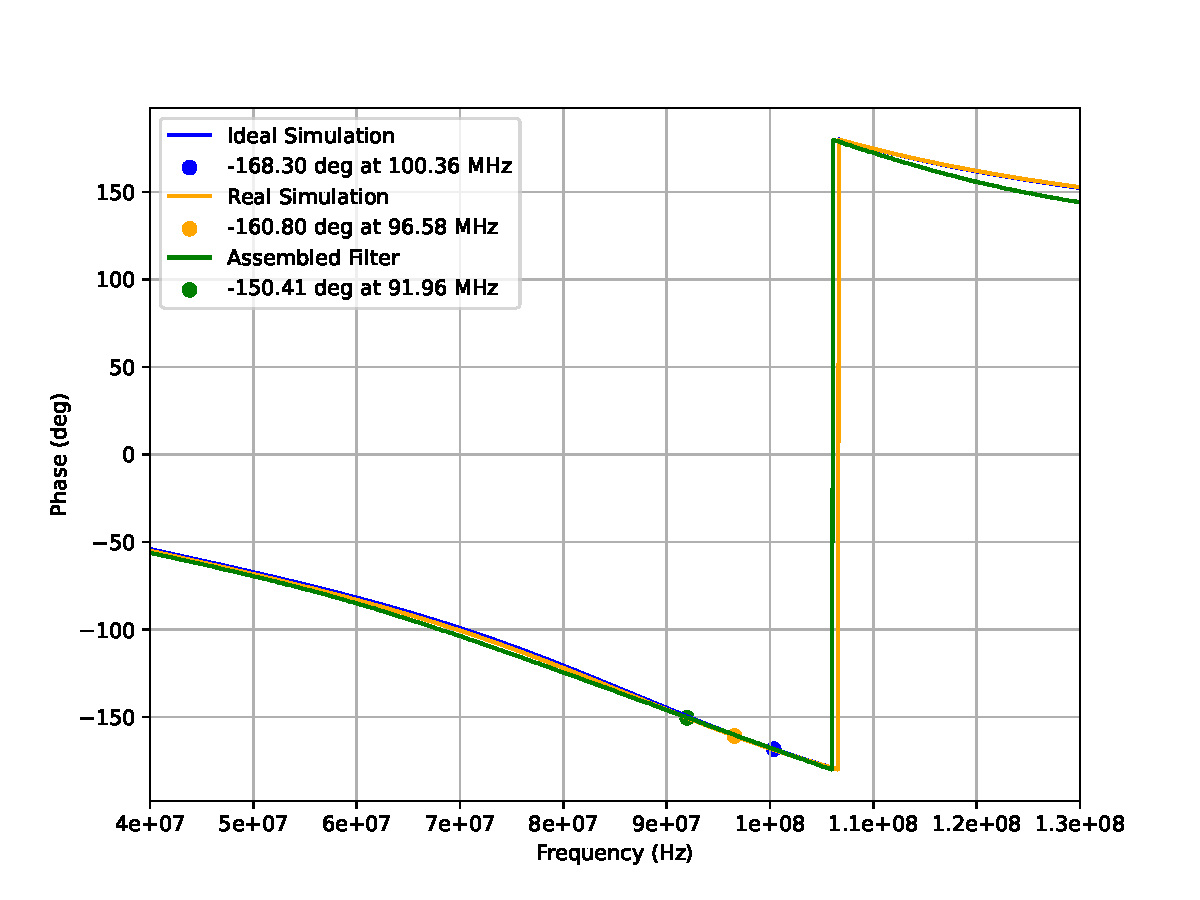
\includegraphics[width=0.7\textwidth]{figures/9.phase_fixed.pdf}
  \caption{S21 phase plot with filter board length adjustment \label{fig:9.phase_fixed}}
\end{figure}
\noindent
Compensating for the extra phase picked up throughout the filter board (assuming phase is picked up like $e^{j\frac{f\cdot 2\pi \cdot 0.5080 \text{ m}}{3\times 10^8 \text{ m/s} \cdot 0.66}}$) we get Figure \ref{fig:9.phase_fixed}, which further confirms that the difference in phase is picked up through the filter PCB.
\\
\\
As expected, the S11 plots also have similar shape (especially the location of the resonant dip). The analytical and ideal simulations both have dips around 90 MHz, while the real simulation and assembled design have dips closer to 80 MHz. The shape of the low frequency falloff differs slightly between the four designs, however it is fairly close for the real and ideal simulations, both of which capture the parsitics ESR that smooths it out.
\\
\\
The S11 and S22 smith charts also match closely between the three designs. Focusing on S21 first (Figure \ref{sec:smith} parts b, d, and f), the swoop shape of all three designs is very similar. The main difference is that the locus touches the unit circle for the ideal simulation while it does not for the real simulation and assembled design. As discussed above this is due to resistive ESR losses and also seen as differences in peak height in Figure \ref{sec:s21_pass}. The loci of the S11 smith charts are also fairly similar (Figure \ref{sec:smith} parts a, c, and e). There is an extra loop in the assembled design at high frequencies. This loop appears to be due to extra phase picked up through the filter board transmission line.
\\
\\
Overall, the four designs match fairly closely. Pass band edge and stop band start for all filters are close to 100 MHz and 174 MHz respectively. In band ripple is the allowed 0.5 dB or less, and insertion loss is less than 0.1 dB for the assembled filter. Additionally, the major difference between simulation and assembled design (the additional phase picked up) can be directly attributed to the size of the filter pcb and it acting like a transmission line.

\subsection{Additional Notes}
All of the data, code, and figures are available in this github repo: \url{github.com/kavidey/e157/tree/main/dp_01}.
\begin{enumerate}
  \item \texttt{predict\_chebyshev.py} generates plots for the analytical design
  \item \texttt{plot\_sim.py} generates plots for the ideal and real simulation (\texttt{sim/} contains the LTSpice \texttt{.asc} files)
  \item \texttt{plot\_data.py} generates plots for the assembled design (\texttt{data/} contains the data from lab)
  \item \texttt{plot\_phase.py} generates the combined phase plot
  \item \texttt{schematics/} has the pretty display schematics made in Altium
\end{enumerate}

\newpage
\section{Takeaways}
% One paragraph about one thing you learned about RF design doing this project.
\indent Prior to working the project I understood the basics of how filter tables, ESR and parasitic impedance worked but this project helped me get a much clearer understanding of how those ideas apply to real world projects.
For example, I didn't realize that amount of desired attenuation the passband edge or corner frequency is ``baked'' into the values of a filter table, and that it is necessary to adjust the corner frequency used in calculation to account for that. When we initially designed our filter, we didn't think about the relationship between maximum ripple \& passband edge and didn't think about the 1 dB vs. 3 dB issue until we tried to analyze our S21 magnitude plot.
Similarly while me and my partner attempted the parasitic extraction process in Lab 3, neither of us understood the full suite of board parasitics (pad capacitance and via inductance) and how they they affected circuits until we had to account for them when designing our ladder filter.

\newpage
\section{Bibliography}
\printbibliography

% referencing bibliography
% ~\cite{melissinos, Cyr, Wiki}

% figures
% \begin{figure}[ht] 
%     \centering \includegraphics[width=0.8\columnwidth]{sr_setup}
%     \caption{
%             \label{fig:samplesetup}
%             Every figure MUST have a caption.
%     }
% \end{figure}

% equations
% \begin{equation} \label{eq:aperp} % the label is used to reference the equation
%     u(\lambda,T)=\frac{8\pi hc\lambda^{-5}}{e^{hc/\lambda kT}-1},
% \end{equation}
%
% ~\ref{fig:samplesetup}

% tables
% \begin{table}[ht]
%     \begin{center}
%         \caption{Every table needs a caption.}
%         \label{tbl:bins} % spaces are big no-no withing labels
%         \begin{tabular}{|cc|}
%             \hline
%             \multicolumn{1}{|c}{$x$ (m)} & \multicolumn{1}{c|}{$V$ (V)} \\
%             \hline
%             0.0044151                    & 0.0030871                    \\
%             0.0021633                    & 0.0021343                    \\
%             0.0003600                    & 0.0018642                    \\
%             0.0023831                    & 0.0013287                    \\
%             \hline
%         \end{tabular}
%     \end{center}
% \end{table}
%
% Table~\ref{tbl:bins} is an example.

% \newpage

% bibliography
% \begin{thebibliography}{99}
%     \bibitem{levitator_paper}
%     Asier Marzo, Adrian Barnes, Bruce W. Drinkwater; TinyLev: A multi-emitter single-axis acoustic levitator. \textit{Rev. Sci. Instrum.} 1 August 2017; 88 (8): 085105. \href{https://doi.org/10.1063/1.4989995}{https://doi.org/10.1063/1.4989995}

%     \bibitem{levitator_instructions}
%     Instructables ultrasonic levitator materials and instructions. \href{https://www.instructables.com/Acoustic-Levitator/}{https://www.instructables.com/Acoustic-Levitator/}
% \end{thebibliography}
\end{document}